% CREATED BY DAVID FRISK, 2016
\chapter{Introduction} \label{ch1}
% CA definition
Concept Alignment (CA) consists in finding semantical correspondences between parts of multilingual parallel texts.
% CA inuition
Such task, often preliminary to further linguistic analysis, is routinely performed by learners of classical languages when working with a translation alongside the original text. It can - and usually does happen simultaneously - at different degrees of abstraction, ranging from word to sentence level. 
While in some cases the student identifies new concepts thanks to language comparison itself (\textit{concept extraction}), there are instances where a set of concepts is already known and the objective becomes finding the corresponding expressions in a certain language (\textit{concept propagation}). \smallskip

% CA in translation 
Another task that involves CA is natural language translation: the human translator, almost subconsciously, first identifies concepts in the source text and only then looks for ways to render them in the target language. 
It is then natural to wonder whether it is possible to make use of CA in Machine Translation (MT) as well.
The hypothesis motivating this project, whose objective is to develop and test strategies for automating CA, is that it can serve as a step of a compositional MT pipeline. 
In such case, its users could easily be provided with a way to verify the correctness of the results by examining - at any level - the ways a concept is expressed in different languages instead of having to compare the entire text in the source language to its automatically translated counterparts.
From this perspective, CA can help develop a more easily interpretable, and therefore more reliable MT system. \smallskip

% motivation
While MT, and in particular Statistical Machine Translation (SMT), does make use of some alignment models, traditional solutions focus on aligning words or, at most, sequences of words, thus generally putting raw strings of text in different languages in relation with each other. This makes it hard to operate at multiple levels of abstraction simultaneously. 
Nevertheless, there are several reasons why a system able to do that is desirable. First of all, choosing the abstraction level to operate at is not trivial, to the point that one could argue that, even within the particular context of translation, correspondences at different levels of abstraction may be more or less useful according to the specific pair of sentences they occur in. 
As an example, let us take the following two English-Italian pairs of sentences: \smallskip

\begin{enumerate}
    \item ``\textit{May I have a piece of cake?}'' and ``\textit{Potrei avere un pezzo di torta?}''
    \item ``\textit{Finding useful correspondences isn't exactly a piece of cake}'' and ``\textit{Trovare corrispondenze utili non è proprio scontato}''
\end{enumerate} \smallskip

In the first case, correspondences on the word level, like ``\textit{piece}''-``\textit{pezzo}'' and ``\textit{cake}''-``\textit{torta}'' are definitely relevant, but in the second sentence pair ``\textit{piece of cake}'' is used idiomatically and it would probably be more useful to just put the whole phrase in relation with ``\textit{scontato}''. \smallskip

\begin{figure}[H]
    \centering
    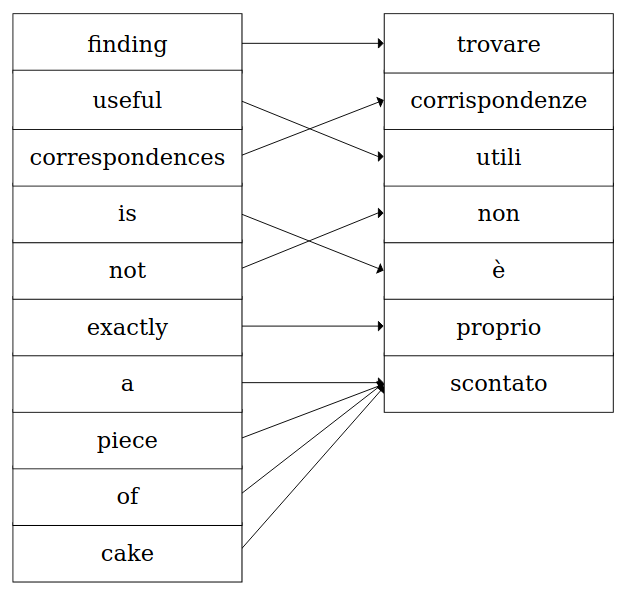
\includegraphics[width=.4\linewidth]{figure/alignment.png}
    \caption[An English sentence aligned with its Italian translation]{An English sentence aligned with its Italian translation. In this case, we are looking for the smallest possible alignments, but it is also possible to find correspondences at a higher level of abstractions, such as ``\textit{useful correspondences}'' and ``\textit{corrispondenze utili}'', which puts two noun phrases in relation with each other.} \label{cake}
\end{figure}

In cases like this, a syntactical comparison between the two sentences can help, if not to extract meaningful correspondences only, which would be the case in the example above, where the complement of the copula ''\textit{is}'' (resp. ``\textit{è}'') is a multiword expression in English and a one-word in Italian, at least to obtain a series of alignments at all levels of abstraction from which to select the most relevant at a later stage\footnote{an example of a more difficult case could be the alternative translation ``Trovare corrispondenze utili non è proprio \textit{un gioco da ragazzi}'', roughly corresponding to ``\textit{a child's play}'' (literally ``\textit{a game (played) by children}''). In this case, trying to align the sentence based on a syntactical comparison would yield both ``\textit{piece of cake}''-``\textit{gioco da ragazzi}'' and the more questionable correspondences ``\textit{piece}''-``\textit{gioco}'' and ``\textit{of cake}-``\textit{da ragazzi}''.}. 
The idea is that, in rule-based MT, using aligned phrases (as opposed to aligned words) is often useful for translating idiomatic expressions correctly and, in general, beneficial in terms of fluency of the output sentences.\smallskip
 
Furthermore, taking syntax into account allows to easily deal with non-contiguous multiword expressions, another situation which is challenging to deal with by means of traditional statistical approaches. For instance, if we consider the sentence ``\textit{Without any linguistic knowledge, it is definitely hard}'' and its Italian translation ``\textit{Senza conoscenze linguistiche, è decisamente arduo}'', a syntactical analysis would make it possible to extract the correspondence ``\textit{is hard}''-``\textit{è arduo}'', even if in both cases the copula and its complement are separated by an adverb. \smallskip

Last but not least, a syntax-based approach can produce correspondences between grammatical objects, as opposed to pairs of strings. Alignments of this kind are valuable, as they can more easily be utilized in rule-based MT systems. \smallskip

% contribution (+ sw deliverables w technologies involved)
With this thesis, we propose a syntax-based approach to both of the above mentioned variants of CA - concept extraction and concept propagation - composed of a neural Universal Dependencies (UD) parser and a rule-based alignment module.
We put our system to the test by integrating it in a prototype domain-specific MT system based on Grammatical Framework (GF).

\section*{Structure of the thesis}
This work is structured as follows. 
Chapter \ref{ch2} gives a few basic definitions, including a more rigorous one of CA itself, as well as providing the necessary background and contextualizing our project by reviewing a few related works. 
Chapters \ref{ch3} and \ref{ch4} focus respectively on extraction and propagation, presenting both our approach to each task and the corresponding experimental results, while Chapter \ref{ch5} describes the experiment designed to produce evaluate how well our CA component performs in the context of MT. 
Finally, Chapter \ref{ch6} consists of a discussion of the overall results and proposes some ideas for future work.